%%%%%%%%%%%%%%%%%%%%%%%%%%%%%%%%%%%%%%%%%%%%%%%%%%%%%%%%%%%%%%%%%%%%%%%%%%%%%%%%%%
% NAME:		swift_scijust_template.tex
% LANGUAGE:	LaTeX
% AUTHOR:	Eleonora Troja, eleonora.troja@nasa.gov
% CREATED:	2014-08-01
% MODIFIED:	2014-08-01
%%%%%%%%%%%%%%%%%%%%%%%%%%%%%%%%%%%%%%%%%%%%%%%%%%%%%%%%%%%%%%%%%%%%%%%%%%%%%%%%%%
%% LaTeX template for the science justification & technical feasibility
%% to be submitted as part of a Swift Guest Investigator proposal.
%%
%% Swift Cycle 11
%% Deadline: 25 September 2014, 4.30pm EDT
%%
%%%%%%%%%%%%%%%%%%%%%%%%%%%%%%%%%%%%%%%%%%%%%%
%%%%% Default format: 11pt single column %%%%%
%%%%%%%%%%%%%%%%%%%%%%%%%%%%%%%%%%%%%%%%%%%%%%

\documentclass[letterpaper,11pt]{article}

\usepackage{graphics,graphicx}
\usepackage{psfig}
\usepackage{times}
\usepackage{amssymb,amsmath}
\usepackage{natbib}
\usepackage{aastexug}

% DO NOT CHANGE THE FOLLOWING 9 LINES!
\setlength{\textwidth}{7in} 
\setlength{\textheight}{9.5in}
\setlength{\topmargin}{-0.2in} 
\setlength{\oddsidemargin}{-0.2in}
\setlength{\evensidemargin}{-0.2in} 
\setlength{\headheight}{0in}
\setlength{\headsep}{0in} 
\setlength{\hoffset}{0in}
\setlength{\voffset}{0in}

\newcommand\ion[2]{#1$\;${\scshape{#2}}}%
\newcommand{\apj}{ApJ}%                                         % Journal abbreviations
\newcommand{\apjs}{ApJS}
\newcommand{\apjl}{ApJL}
\newcommand{\aap}{A{\&}A}
\newcommand{\aaps}{A{\&}AS}
\newcommand{\mnras}{MNRAS}
\newcommand{\aj}{AJ}
\newcommand{\araa}{ARAA}
\newcommand{\pasp}{PASP}
\newcommand{\nat}{Nature}
\newcommand{\sci}{Science}
\newcommand{\spie}{Proc.~of SPIE}
\newcommand{\arcsec}{\mbox{$^{\prime\prime}$}}% 
\newcommand{\arcmin}{\mbox{$^\prime$}}% 

\makeatletter
\renewcommand{\section}{\@startsection%
{section}{1}{0mm}{-\baselineskip}%
{0.5\baselineskip}{\normalfont\Large\bfseries}}%
\makeatother

%%%%%%%%%%%%%%%%%%%%%%%%%%%%%%%%%%%%%%%%%%%%%%%%%%%%%%%%%%%%%%%%%%%%%%%%%%%%%%%%%%
%  NOTES:
% 
%  - THE SCIENTIFIC JUSTIFICATION MUST NOT EXCEED 4 PAGES!
%     (The only exception are proposals in the "high redshihft GRB" category which can have up to 6 pages
%
%  - THE "BUDGET NARRATIVE" MUST BE LESS THAN 1 PAGE AND DOES  NOT  COUNT TOWARD THE ABOVE PAGE LIMIT
%
%  - THE FONT CANNOT BE SMALLER THAN 11pt
%
%  - Do NOT include a CV, current and pending support, or amny other supporting information 
%
%  - THE SCIENTIFIC JUSTIFICATION MUST BE SUBMITTED AS  PDF  FILE:
%
%  latex swift_scijust_template.tex
%  dvips swift_scijust_template -o swift_scijust_template.ps
%  ps2pdf swift_scijust_template.ps swift_scijust_template.pdf
%
%%%%%%%%%%%%%%%%%%%%%%%%%%%%%%%%%%%%%%%%%%%%%%%%%%%%%%%%%%%%%%%%%%%%%%%%%%%%%%%%%%

\begin{document}
\pagestyle{plain}
\pagenumbering{arabic}

\begin{center} 
\bfseries\uppercase{The Rapid IMAger and Spectrograph (RIMAS): A New Window
	into the High-Redshift Universe}
\end{center}
\vspace{-0.3cm}
\centerline{\bf PI: {A. Kutyrev}}
 
\noindent {\bf 1. Abstract}
\smallskip\\
RIMAS is a new NIR instrument designed expressly to identify high-redshift 
$\gamma$-ray bursts (GRBs) from \textit{Swift} within minutes, scheduled to be installed on the 
4.3\,m Discovery Channel Telescope (DCT) in first half of 2015. RIMAS can operate in and switch 
rapidly (10s of seconds) between three modes: 1) Simultaneous 2-band imaging; 2) High-throughput, $R \approx 25$ 
NIR spectroscopy; 3) High-resolution ($R \approx 4500$), cross-dispersed echelle spectroscopy providing 
simultaneous coverage from 0.9--2.4\,$\mu$m. Unlike other large aperture facilities that 
are classically scheduled, RIMAS will be continuously available for automated ToO observations 
through a dichroic beamsplitter that allows simultaneous coverage with an optical imager, 
the Large Monolithic Imager (LMI). By the end of cycle 11, we intend for RIMAS to be routinely 
obtaining rapid multi-color photometry and NIR spectra of Swift afterglows to measure 
their redshifts and constrain properties of their host galaxies and the surrounding 
IGM. \\

\noindent {\bf 2. Description of the Proposed Program}
\smallskip\\
\noindent {\it A) Scientific Rationale:}
\smallskip\\
Understanding both the precise time history and the sources responsible for cosmic
reionization remains one of the most sought-after goals of modern cosmology.  The 
discovery of Gunn-Peterson troughs in the spectra of $z \gtrsim 6$ quasars 
(QSOs\cite{bfw+01}) seemed to imply at least a modest neutral H fraction 
($x_{\mathrm{H\,I}}$) at this time.  However, observations of the cosmic microwave
background (CMB\cite{hlk+13}) indicate a significantly larger characteristic redshift 
for reionization to occur: $z_\mathrm{reion} \approx 10$.  It may be 
possible to reconcile these two seemingly contradictory observations if reionization
were to occur slowly, with a large degree of small-scale variation.  But many more
sightlines are needed to test this hypothesis, something not possible for QSOs
with current instrumentation.

While both QSOs and the CMB have been used to study reionization for some time, 
long-duration $\gamma$-ray bursts (GRBs) are a relatively new probe of the high-redshift 
universe (e.g., \cite{lr00}).  GRBs offer several theoretical advantages over QSOs
for constraining $x_{\mathrm{H\,I}}$ near the epoch of reionization: 1) Though
short-lived, their afterglow emission can significantly outshine even the brightest
QSOs (e.g., \cite{rks+08,bpl+09,kmk07}); 2) The power-law afterglow spectral energy 
distributions are significantly simpler to model than QSOs, leading to more precise 
$x_{\mathrm{H\,I}}$ measurements \cite{mlz+08}; 3) Because they result from the 
core-collapse of a single massive star, GRBs are not biased towards the most massive halos\cite{mlz+08}.

Thanks to more than a decade of painstaking effort from the community, we are finally
on the cusp of using GRBs to make meaningful measurements of the neutral H fraction 
at cosmologically interesting redshifts ($z \gtrsim 7$).  The discovery of 
GRB\,090423 at $z \approx 8.2$ \cite{tfl+09,sdc+09}, the most distant 
spectroscopically confirmed source in the universe (Figure 1), along with the 
measurement of a photometric redshift of $z \sim 9.4$ for GRB\,090429B \cite{clf+11}, 
unambiguously establish that GRBs explode and are detectable at the relevant redshifts 
of interest.  In fact we have relatively precise constraints on the rate of such events from 
unbiased \textit{Swift} samples: $\approx$ a few percent of the \textit{Swift} population 
resides at $z \gtrsim 7$ (1--2 events per year; \cite{pcb+09,gkk+11}).  Furthermore, 
high signal-to-noise ratio (SNR) spectroscopy of the $z = 5.913$ GRB\,130606A (Figure 1) 
enabled for the first time a strict upper limit on the neutral H fraction of $x_{\mathrm{H\,I}} < 0.11$ 
from the lack of a Ly$\alpha$ red damping wing \cite{cbf+13}.

%-----------------------------Figure Start------------------------------
\begin{figure}[tp!]
\begin{center}
\hbox{
% un-comment the following line to include your fig1a.ps postscript file:
%\psfig{figure=figures/Slide1.jpg,height=4.0cm,width=8.0cm,angle=0}
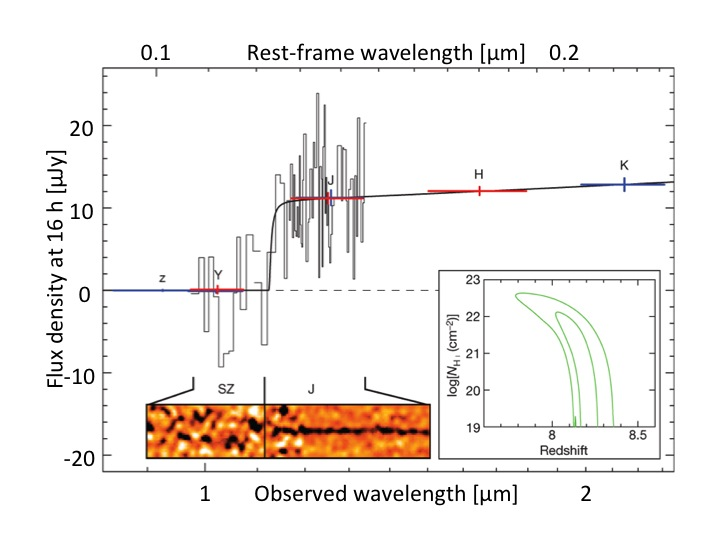
\includegraphics[width=0.47\textwidth]{figures/Slide1.jpg}
\hspace{0.5cm}
% un-comment the following line to include your fig1b.ps postscript file:
%\psfig{figure=fig1b.ps,height=4.0cm,width=7.0cm,angle=0}
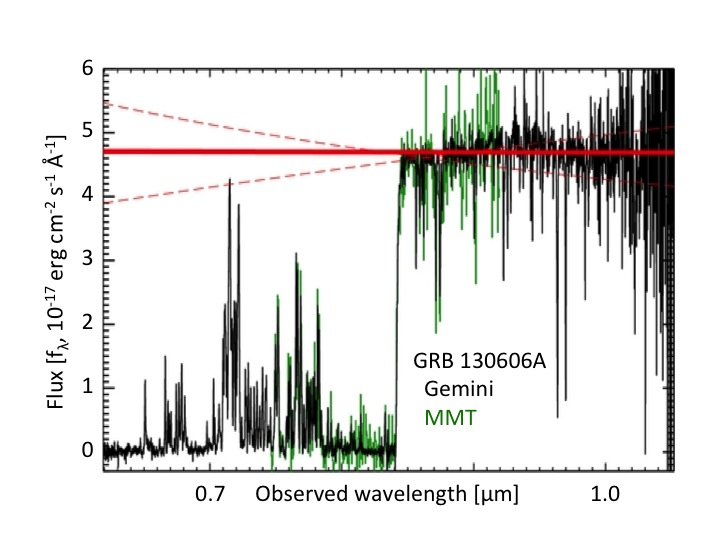
\includegraphics[width=0.47\textwidth]{figures/Slide2.jpg}
}
\vspace{-0.9cm}
\end{center}
\caption{\footnotesize
{{\it Left panel}: NIR spectrum of the afterglow of the $z = 8.2$ 
GRB\,090423\cite{tfl+09}, obtained with ISAAC on the VLT at full 16\,hr
after the burst trigger time.  While the sharp break in the spectrum (consistent
with that obtained from broadband photometry) indicates a redshift of $z \approx
8.2$, the low SNR precludes meaningful constraints on $x_{\mathrm{H\,I}}$.
{\it Right panel}: Optical spectra of the $z = 5.913$ 
GRB\,130606A\cite{cbf+13}.  The sharp
drop in flux blueward of $\sim 8300$\,\AA\ is due to absorption from neutral H
in the host galaxy and intervening IGM.  Modeling the red wing of the Ly$\alpha$
absorption enabled the first constraints on $x_{\mathrm{H\,I}}$ 
comparable to what has been obtained
from QSOs at $z \approx 6$.  However, thus far, no high SNR spectra of a GRB
afterglow has been obtained at a redshift directly probing the epoch 
of reionization ($z \gtrsim 7$).}}
\label{fig1}
\end{figure}
%-----------------------------Figure End--------------------------------


Despite these remarkable successes, as a community we still lack the ultimate
prize: meaningful constraints on $x_{\mathrm{H\,I}}$ at a redshift of interest
for reionization ($z \gtrsim 7$).  Given that \textit{Swift} has likely detected
$\gtrsim 10$ events over the course of its lifetime at these distances, the
bottleneck is clear: a lack of promptly available NIR imaging and spectroscopy 
on moderate / large aperture telescopes.  At $z \gtrsim 7$, rest-frame Ly$\alpha$
is redshifted into the observer-frame NIR.  While many promptly available 
optical facilities automatically respond to \textit{Swift} GRB alerts, the number
of \textit{readily available} NIR imagers, and, to an even larger degree,
spectrographs, is remarkably small [RATIR, GROND, NIRI (Gemini), X-SHOOTER (VLT)].
Without NIR capabilities, it is nearly impossible to distinguish between events
that are optically faint because they are obscured by dust (a significant fraction
of the \textit{Swift} population; \cite{ckh+09,pcb+09,gkk+11}) and true
high-redshift GRBs, let alone measure $x_{\mathrm{H\,I}}$ from the red wing of
Ly$\alpha$.

Here we request funding to assist with the commissioning of the Rapid infrared
IMAger and Spectrograph (RIMAS), a new NIR imager and spectrograph to be installed and 
\textit{continuously available} on the 4.3\,m Discovery Channel Telescope (AZ) in early 
2015.

\smallskip

\noindent {\it B) Immediate Objective:}
\smallskip\\
Our principle objective is quite straightforward: by the end of Cycle 11, we intend
for RIMAS to be routinely obtaining rapid multi-color photometry and (as appropriate) 
NIR spectroscopy of \textit{Swift} afterglows to measure their redshifts and constrain 
properties of their host galaxies and the surrounding IGM.  To better understand the 
level of effort required to reach this point, we first provide an overview of the 
instrument design and a summary of the current status.

\smallskip

\noindent{\underline{Design Overview:}}
RIMAS is a collaborative effort between Goddard Space Flight Center, the University of
Maryland, and Lowell Observatory.  The instrument is being designed for the recently
commissioned 4.3\,m Discovery Channel Telescope (DCT).  RIMAS will be installed on one 
port of the DCT ``instrument cube'', where a dichroic beamsplitter will allow users to
switch between multiple instruments with an overhead of only seconds and simultaneously
image with LMI.

RIMAS has three operating modes: imaging, low spectral resolution (R $\approx 25$) and
a high resolution mode ($R \approx 4500$). The spectral coverage spans from 
0.9--2.4\,$\mu$m ($Y$-, $J$-, $H$-, and $K$-band).  The optical layout has two arms 
with two detectors allowing for a simultaneous imaging in two bands, $Y$ or $J$ in 
one arm of the instrument, and $H$ or $K$ in the other.  The designed ensquared
energy is near the diffraction limit, with one pixel corresponding to 0.35\arcsec, 
and a field-of-view of 3\arcmin $\times$ 3\arcmin.  With its broad spectral coverage 
and both imaging and spectral modes available, RIMAS will be a powerful tool for 
both rapid (within minutes) photometric and spectroscopic follow-up of \textit{Swift} GRBs.

\smallskip

\noindent{\underline{Design Details:}}
A drawing of the optical and mechanical layout of RIMAS is shown in Figure~2.
Before entering the main dewar, the beam enters a front module, an attachment to the 
dewar operating at $\approx 60$\,K under vacuum. The attachment contains field-limiting 
slits, which can be placed at the focus of the telescope for use with the 
dispersive elements. Slits of various sizes or an open slot for photometry can be selected by 
rotating a slit wheel. The surface of each slit is a mirror that reflects light into a slit-imaging 
camera (with 256 x 256, 80\arcsec\ diameter IR detector) to help observers center light from 
their source through the slit.  The slit-wheel will have a pick-off mirror for the future 
installation of MOHSIS, a fiber-Bragg grating (FBG) atmospheric hydroxyl (OH) emission 
line suppressor. Behind the slit-wheel, there is a  filter wheel for program-specific specialty filters. 

%-----------------------------Figure Start------------------------------
\begin{figure}[tp!]
\begin{center}
\hbox{
% un-comment the following line to include your fig1a.ps postscript file:
%\psfig{figure=fig1a.ps,height=4.0cm,width=8.0cm,angle=0}
\includegraphics[width=0.47\textwidth]{figures/slide3.jpg}
\hspace{0.5cm}
% un-comment the following line to include your fig1b.ps postscript file:
%\psfig{figure=fig1b.ps,height=4.0cm,width=7.0cm,angle=0}
\includegraphics[width=0.47\textwidth]{figures/slide4.jpg}
}
\vspace{-0.7cm}
\end{center}
\caption{\footnotesize
{{\it Left panel}: The layout of the optical and mechanical elements used in RIMAS.
Light from the DCT first passes through the filter and slit wheels in the 
front module, is collimated and continues until focused by the ``YJ-band'' 
(0.9--1.4\,$\mu$m) or ``HK-band'' (1.4--2.4\,$\mu$m) camera.
{\it Right panel}: A photo of RIMAS in the lab at Goddard Space Flight Center.}}
\label{fig2}
\end{figure}
%-----------------------------Figure End--------------------------------

All of the optics are kept cold ($T \approx 60$\,K) to reduce 
thermal background, which is crucial at the long end of the instrument’s 
wavelengths in $K$-band. The beam is separated into two optical arms by a
dichroic beamsplitter. The first arm is for the $Y$- and $J$-bands 
(0.97--1.07 and 1.17--1.33\,$\mu$m, respectively), and the second is for the $H$- 
and $K$-bands (1.49-1.78 and 2.03--2.37\,$\mu$m, respectively). Each 
arm has a filter wheel that holds broadband photometric filters as well as low ($R \approx
25$) and high ($R \approx 4500$) spectral resolving power diffractive elements. 
The wheels allow the observer or automation software to switch between instrument modes 
within seconds.  The light of each arm will be focused onto a Teledyne HAWAII-2RG (H2RG) detector.

High resolution spectroscopy will be achieved for each optical arm by using 
multiple, cross-dispersed orders of transmission gratings (Figure~3).  RIMAS
can change modes in 10s of seconds.

\smallskip

\noindent{\underline{Expected Performance:}}
Based on the pre-commissioning calculations of the system throughput, we estimate 
the following 10$\sigma$ limiting magnitudes (AB) will be achieved in a 400\,s
integration in imaging mode for a point source obtained under good 
conditions: $Y > 22.1$, $J > 22.0$, $H > 21.2$, $K > 20.7$.  Limiting
magnitudes for a 1\,hr integration using the low-resolution ($R \approx 25$)
spectral mode are very similar to these imaging limits.  For comparison, 
these values are $\gtrsim 1.5$\,mag deeper in all filters than those typically 
achieved by e.g., GROND, in their prompt follow-up GCNs.

Similarly, we estimate we will be able to achieve a SNR per resolution element of 
10 in a 1\,hr exposure in the high-resolution echelle mode with the 0.6\arcsec\ 
slit for sources with the following (AB) magnitudes: $Y = 18.1$, $J = 17.6$, 
$H = 16.1$, and $K = 15.2$.  After correcting for comparable SNRs and slit
widths, these sensitivities are comparable to analogous instruments on 
similar-sized telescopes, e.g., TripleSpec on the Palomar 200\,inch telescope, and
TripleSpec on the 3.5\,m ARC telescope.

\smallskip

\noindent{\underline{Rapid Response Expected Performance:}}
We expect that RIMAS will be able to begin spectroscopy within 5 minutes of a bright GRB trigger.
We observed GRB140215A on DCT with LMI and were able to get on source 
within 3 minutes of the \textit{Swift} trigger manually.  We expect this response time will be significantly reduced with 
automation software.  RIMAS's automation software will take short exposure images and 
decide whether it should continue with longer exposure images or if the source is bright 
enough to switch to either low- or high- resolution spectroscopy.

We estimate 3$\sigma$ limiting magnitudes (AB) in 30\,s integration 
in imaging mode for a point source obtained under good conditions: 
$Y > 22.1$, $J > 22.1$, $H > 21.3$, $K > 20.9$.  For a bright source that means RIMAS can
follow-up in less than 5 minutes.  The automation software will get a magnitude estimate and 
choose between low- and high- resolution spectroscopy based on limiting magnitude calculations.
This will allow RIMAS to obtain spectroscopy rapidly before the afterglow has faded beyond detection limits.

%-----------------------------Figure Start------------------------------
\begin{figure}[tp!]
\begin{center}
% un-comment the following line to include your fig1a.ps postscript file:
%\psfig{figure=fig1a.ps,height=4.0cm,width=8.0cm,angle=0}
\includegraphics[width=0.47\textwidth]{figures/slide5.jpg}
\vspace{-0.7cm}
\end{center}
\caption{\footnotesize
{ Estimated instrument photometric efficiency}}
\label{fig2}
\end{figure}
%-----------------------------Figure End--------------------------------

\smallskip

\noindent{\underline{Project Status:}}
The RIMAS instrument is currently in the process of assembly at GSFC (Figure~2).
The dewar has passed all cryo-mechanical tests in the lab.  We have acquired both of the H2RG detectors (for the Y/J 
arm and the H/K arm), as well as the detector drive and image acquisition electronics
(Leach-based).  We are currently characterizing the detectors in RIMAS's dewar.

All optics excluding the gratings and two out of the four broadband filters have been received and characterized.  
The guide camera has been aligned at room temperature while science optics remain to be AR 
coated before aligned in their mounts at room temperature. We are working with Lawrence Livermore 
National Laboratory (LLNL) to produce the required dispersive elements (gratings).  

The mechanical structure is partially built (e.g., the internal optical bench and 
the detector mounts).  We have half of the opto-mechanical components and the other half 
are currently being fabricated.   We expect all of the necessary 
hardware tasks will have been completed by the commencement of Cycle 11 (1 April 2015), 
and the instrument will be shipped for installation on the DCT around this time.

\smallskip

\noindent{\underline{Remaining Tasks:}}
While the hardware design, acquisition, and integration is underway and largely 
funded, our experience with RATIR, P60, etc.~indicate that our software needs will
be significant.  In particular, the bulk of our requested funding is dedicated to 
two major software efforts:
\begin{itemize}
\item We request funding for a professional programmer to handle the low-level (e.g.,
C++ level) software to control the instrument and interface with the DCT.  This 
effort would include routine operations (e.g., selecting instrument configuration,
writing out resulting exposures with appropriate FITS header keywords), as well as 
the development of a rapid-response mode suitable for automated multi-color 
follow-up and (as appropriate) spectroscopy of \textit{Swift} GRBs.
\item We also request funding for a graduate student to develop higher-level (e.g.,
python) analysis tools to promptly reduce both the imaging and spectroscopic outputs
into fully processed data products (i.e., a pipeline) and automation software to allow 
RIMAS to quickly decide between its operating modes.    
\end{itemize}
A more detailed budget is provided in the Budget Narrative section at the end of 
this proposal.\\



\noindent {\bf 3. Justification of Requested Observing Time, Feasibility and Visibility}
\smallskip\\
We are not requesting any additional \textit{Swift} observations for this program.
Instead we estimate the number of GRBs we will be able to observe
with RIMAS when it is fully operational; how many we will detect (photometrically) and 
how many we will follow up spectroscopically (e.g. redshifts). 

Based on our past experience with robotic follow-up of \textit{Swift} GRBs (P60,
RATIR), we anticipate that $\approx 10$ GRBs will be promptly ($\Delta t < 1$\,hr) 
observable to the DCT over the course of Cycle 11.  An additional 20--30 events will 
be observable within 1\,d of the burst trigger time.

We can estimate our detection efficiency using the sample of with prompt ($\Delta t
< 1$\,d) with the GROND instrument on the MPI/ESO 2.2\,m telescope on La Silla 
(Chile)\cite{gkk+11}.  Using their simultaneous 7-color imager, these authors report
recovering $\approx$ 90\% of GRBs observed within 1\,hr, and $\approx$ 60\% of
GRBs observed within 1\,d.  Given that RIMAS on the 4.3\,m DCT is expected to be
$\approx 1.5$\,mag more sensitive in the NIR than GROND, these recovery fractions 
represent extremely conservative lower limits for what we can expect with RIMAS. 
We therefore expect to detect (via broadband imaging) $\gtrsim 30$ GRB afterglows.

Nearly all of the events we detect via broadband imaging will be sufficiently 
bright to obtain low-resolution ($R \approx 25$) spectra.  This will allow crude
spectroscopic estimates for all events at $z \gtrsim 6.5$ via the detection of a
Ly$\alpha$ break, and upper redshift limits (from the lack of a Ly-break)
for \textit{all events detected by RIMAS.}  Based on the relative rate of 
high-redshift GRBs in the \textit{Swift} sample\cite{pcb+09,gkk+11}, we expect 
to detect $\approx 1$ GRB at $z \gtrsim 7$, and several events at $z \gtrsim 5$ 
each year. 

It is difficult to reliably predict how many events will be suitably bright 
for high-resolution spectroscopy with RIMAS.  For simplicity, we can compare with known
high-redshifts events.  GRB\,090423\cite{tfl+09} was observed at $K = 18.0$\,mag at
$\Delta t = 40$\,min, and $J = 19.2$\,mag at $\Delta t = 80$\,min.  Both filters are 
sufficiently bright that we could obtain modest SNR ($\approx 5$ per resolution
element) with a 1\,hr integration with RIMAS.  Similarly, GRB\,050904\cite{hnr+05}
was observed with $J = 18.3$\,mag at $\Delta t = 3$\,hr, and $K = 18.6$\,mag as
late as $\Delta t = 8$\,hr after the burst trigger.  If observed promptly, it is likely
GRB\,050904 could have been well-detected by RIMAS.

Our collaboration has observed GRB afterglows at visible wavelengths during 4 separate, one week runs (non-ToO) using Large Monolithic Imager (LMI) on DCT. To date we have observed 12 GRB afterglows with 9 accompanying GCN circulars (Table \ref{table:DCTobs}), demonstrating the quality of the site and telescope. Additionally, we were able to begin observing GRB140215A 2.7 minutes post-bust without any automation software.  We expect that we will be able to do much better once RIMAS has been commissioned and automated. \\

	\begin{table}[ht]
		\centering 
		\begin{tabular}{lll}
			\hline\hline
			\textbf{Swift name} & \textbf{Detected?} & \textbf{GCN circulars}		\\
			\hline
			GRB140129A			& No					&							\\
			GRB140209A			& No					&							\\
			GRB140206A			& Yes					& 15835						\\
			GRB140215A			& Yes					& 15838, 15850				\\
			GRB140311A			& No					&							\\
			GRB140318A			& Yes					& 15989						\\
			GRB140606A			& Yes					& 16367, 16377				\\
			GRB140606B			& No					&							\\
			GRB140610A			& No					&							\\
			GRB140614B			& No					&							\\
			GRB140903A			& Yes					& 16769, 16785				\\
			GRB140907A			& Yes					& 16802, 16818				\\
			\hline
		\end{tabular}
		\caption{GRB observations with DCT-LMI}
		\label{table:DCTobs} 
	\end{table}

\noindent {\bf 4. Justification of Duplication}
\smallskip\\
We are not requesting a duplicate accepted proposal.\\

\noindent {\bf 5. Report on Previous Swift and Related Programs}
\smallskip\\
This is our first request specifically for funding for RIMAS.  In previous cycles,
several members of our collaboration received \textit{Swift} GI funding for the 
construction and commissioning of RATIR, a simultaneous 4-band optical and NIR
imager mounted on the 1.5\,m Johnson telescope on Sierra San Pedro Martir in Baja 
California.  RATIR now routinely observes \textit{Swift} GRB afterglows, publishing
$>$ 100 GCNs over the past 2 years, with 6 refereed journal publications and 
many others in the preparation stage. \\

\noindent {\bf 6. References}
\smallskip\\
{\footnotesize

%%%%%
%Capone, J. I. et al., 2013, \spie, 8863, 8863-14: \textit{The development and 
%analysis of cryogenic optical systems for the rapid infrared imager/spectrometer} \\
%Butler, N. R. et al., 2012, \spie, 8446, 8446-10: \textit{First Light with RATIR: 
%an Automated 6-band Optical/NIR Imaging Camera} \\
%Cenko, S. B. et al., 2006, \pasp, 118, 1396: \textit{The Automated Palomar 
%60 Inch Telescope} \\
%Cenko, S. B. et al., 2009, \apj, 693, 1484: \textit{Dark Bursts in the Swift Era: 
%The P60-Swift Early Optical Afterglow Catalog} \\
%Perley, D. A. et al., 2009, \aj, 138, 1690: \textit{The Host Galaxies of Swift Dark 
%Gamma-Ray Bursts: Observational Constraints on Highly Obscured and Very High-Redshift 
%GRBs} \\
%Tanvir, N. R. et al., 2009, \nat, 461, 1264: \textit{A gamma-ray burst at a redshift 
%of 8.2} \\
%Haislip, J. B. et al., 2006, \nat, 440, 181: \textit{A photometric redshift of 
%$z = 6.39 \pm 0.12$ for GRB\,050904} \\
%Morgan, A. N. et al., 2013, \mnras\ submitted (astro-ph/1305.1928): \textit{Evidence 
%for Dust Destruction from the Early-time Colour Change of GRB 120119A} \\
%Perley, D. A. et al., 2013, \apj\ submitted (astro-ph/1301.5903): \textit{A 
%Population of Massive, Luminous Galaxies Hosting Heavily Dust-Obscured 
%Gamma-Ray Bursts: Implications for the Use of GRBs as Tracers of Cosmic Star 
%Formation} \\
%Svensson, K. M. et al., 2012, \mnras, 421, 25: \textit{The dark GRB 080207 in an 
%extremely red host and the implications for gamma-ray bursts in highly 
%obscured environments} \\
%Perley, D. A. et al., 2011, \aj, 141, 36: \textit{Monster in the Dark: The 
%Ultraluminous GRB 080607 and Its Dusty Environment} \\
%Cenko, S. B. et al., 2010, \aj, 140, 224: \textit{Unveiling the Origin of 
%GRB\,090709A: Lack of Periodicity in a Reddened Cosmological Long-Duration 
%Gamma-Ray Burst} \\
%%%%%

\bibliographystyle{nature.bst}
%\bibliography{rimas.cy11.bib}
}

\clearpage

\noindent {\bf 7. Budget Narrative}
\smallskip\\
Costs are summarized in the table below and are fully loaded, i.e., salaries include
fringe benefits and all necessary items include appropriate institutional overheads.
The components of the cost are:
\begin{itemize}
\item 4 months of effort (0.3 FTE) from a professional software engineer to provide
the low-level tools to control the instrument and interface with the DCT.  We plan
to hire this individual as a (short-term) contractor at GSFC, for an estimated total
cost of \$40k.
\item 6 months of effort (0.5 FTE) from 1--2 University of Maryland graduate students
to develop a data reduction pipeline for RIMAS.  In order to make intelligent
decisions regarding the appropriate follow-up strategy for \textit{Swift} GRBs in
real-time (i.e., broadband imaging or spectroscopy), the pipeline will need to be
capable of prompt reductions (at least with preliminary calibrations).  A more 
precise and robust pipeline for science-quality reductions, of obvious utility 
for the entire RIMAS user base, can be executed in a more leisurely manner (but will
also be developed by these students).  We estimate a total cost for this effort 
of \$25k.
\item 1 month of effort (0.1 FTE) for PI Kutyrev to oversee the effort,
including the installation of the hardware on the DCT, as well as supervising the
professional programmer and graduate student(s) in software development.  The 
total cost of his effort will be \$10k.
\item 1 month of effort (0.1 FTE) for co-I Norris, to assist in the theoretical
interpretation of early RIMAS results, in particular relating $x_{\mathrm{H\,I}}$
measurements from RIMAS to previously observed QSOs as well as in the broader 
context of reionization physics.
\item \$10k for travel, including multiple trips for team members (Kutyrev, Cenko,
and graduate students) to Flagstaff, AZ (location of the DCT) for instrument 
installation and/or upgrades, as well as for co-I Norris to visit GSFC to work 
with the team on interpreting the observations.
\item \$5k for publishing our results, including journal pages charges (e.g., \apj),
as well as for 1--2 team members (preferably graduate students) to travel to 
scientific conferences to present our results.
\end{itemize}

The total request cost thus comes to \$100k, with a total FTE request of 1.0.

\smallskip

\begin{center}
\begin{tabular}{lc}
\multicolumn{2}{c}{\textbf{Projected Costs}} \\
\hline
Professional Software Development & 40k \\
Graduate Student Pipeline & 25k \\
Kutyrev Oversight & 10k \\
Norris Theoretical Interpretation & 10k \\
Travel (DCT Commissioning, Upgrades) & 10k \\
Publications (Page Charges, Conference) & 5k \\
\hline
\textbf{Total Cost} & \textbf{100k} \\
\end{tabular}
\end{center}

%-----------------------------Figure Start------------------------------
%\begin{figure}[htp!]
%\begin{center}
%\hbox{
%%uncomment the following line to include your fig1a.ps postscript file:
%\psfig{figure=fig1a.ps,height=4.0cm,width=8.0cm,angle=0
%}
%\hspace{0.5cm}
% un-comment the following line to include your fig1b.ps postscript file:
%\psfig{figure=fig1b.ps,height=4.0cm,width=7.0cm,angle=0}
%}
%\end{center}
%\caption{\footnotesize
%{{\it Left panel}: here you see...
%{\it Right panel}: here you see...}}
%\label{fig1}
%\end{figure}
%-----------------------------Figure End--------------------------------


\end{document}
